% Created by tikzDevice version 0.12.3.1 on 2021-12-03 16:28:28
% !TEX encoding = UTF-8 Unicode
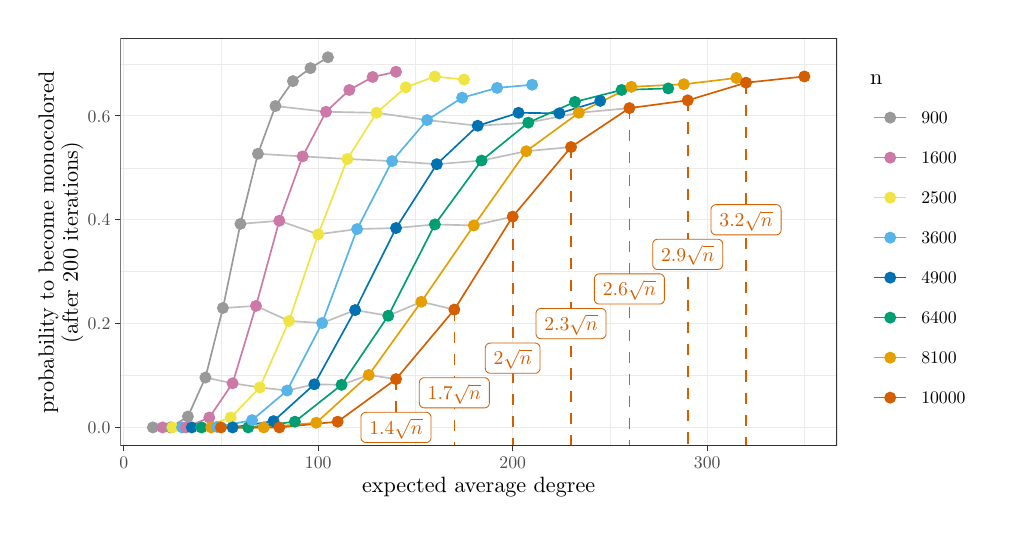
\begin{tikzpicture}[x=1pt,y=1pt]
\definecolor{fillColor}{RGB}{255,255,255}
\path[use as bounding box,fill=fillColor,fill opacity=0.00] (0,0) rectangle (346.90,173.45);
\begin{scope}
\path[clip] (  0.00,  0.00) rectangle (346.90,173.45);
\definecolor{drawColor}{RGB}{255,255,255}
\definecolor{fillColor}{RGB}{255,255,255}

\path[draw=drawColor,line width= 0.4pt,line join=round,line cap=round,fill=fillColor] (  0.00,  0.00) rectangle (346.90,173.45);
\end{scope}
\begin{scope}
\path[clip] ( 33.48, 22.32) rectangle (292.45,169.45);
\definecolor{fillColor}{RGB}{255,255,255}

\path[fill=fillColor] ( 33.48, 22.32) rectangle (292.45,169.45);
\definecolor{drawColor}{gray}{0.92}

\path[draw=drawColor,line width= 0.2pt,line join=round] ( 33.48, 47.76) --
	(292.45, 47.76);

\path[draw=drawColor,line width= 0.2pt,line join=round] ( 33.48, 85.28) --
	(292.45, 85.28);

\path[draw=drawColor,line width= 0.2pt,line join=round] ( 33.48,122.80) --
	(292.45,122.80);

\path[draw=drawColor,line width= 0.2pt,line join=round] ( 33.48,160.32) --
	(292.45,160.32);

\path[draw=drawColor,line width= 0.2pt,line join=round] ( 69.85, 22.32) --
	( 69.85,169.45);

\path[draw=drawColor,line width= 0.2pt,line join=round] (140.12, 22.32) --
	(140.12,169.45);

\path[draw=drawColor,line width= 0.2pt,line join=round] (210.40, 22.32) --
	(210.40,169.45);

\path[draw=drawColor,line width= 0.2pt,line join=round] (280.67, 22.32) --
	(280.67,169.45);

\path[draw=drawColor,line width= 0.4pt,line join=round] ( 33.48, 29.00) --
	(292.45, 29.00);

\path[draw=drawColor,line width= 0.4pt,line join=round] ( 33.48, 66.52) --
	(292.45, 66.52);

\path[draw=drawColor,line width= 0.4pt,line join=round] ( 33.48,104.04) --
	(292.45,104.04);

\path[draw=drawColor,line width= 0.4pt,line join=round] ( 33.48,141.56) --
	(292.45,141.56);

\path[draw=drawColor,line width= 0.4pt,line join=round] ( 34.71, 22.32) --
	( 34.71,169.45);

\path[draw=drawColor,line width= 0.4pt,line join=round] (104.99, 22.32) --
	(104.99,169.45);

\path[draw=drawColor,line width= 0.4pt,line join=round] (175.26, 22.32) --
	(175.26,169.45);

\path[draw=drawColor,line width= 0.4pt,line join=round] (245.54, 22.32) --
	(245.54,169.45);
\definecolor{drawColor}{RGB}{190,190,190}

\path[draw=drawColor,line width= 0.6pt,line join=round] ( 64.23, 47.01) --
	( 74.06, 44.95) --
	( 83.90, 43.45) --
	( 93.74, 42.32) --
	(103.58, 44.58) --
	(113.42, 44.39) --
	(123.26, 47.95) --
	(133.10, 46.45);

\path[draw=drawColor,line width= 0.6pt,line join=round] ( 70.55, 72.15) --
	( 82.50, 72.90) --
	( 94.44, 67.46) --
	(106.39, 66.71) --
	(118.34, 71.40) --
	(130.29, 69.34) --
	(142.23, 74.40) --
	(154.18, 71.59);

\path[draw=drawColor,line width= 0.6pt,line join=round] ( 76.88,102.54) --
	( 90.93,103.67) --
	(104.99, 98.79) --
	(119.04,100.67) --
	(133.10,101.04) --
	(147.15,102.35) --
	(161.21,101.98) --
	(175.26,105.17);

\path[draw=drawColor,line width= 0.6pt,line join=round] ( 83.20,127.87) --
	( 99.36,126.93) --
	(115.53,125.99) --
	(131.69,125.24) --
	(147.85,124.12) --
	(164.02,125.43) --
	(180.18,128.81) --
	(196.34,130.31);

\path[draw=drawColor,line width= 0.6pt,line join=round] ( 89.53,145.13) --
	(107.80,143.06) --
	(126.07,142.69) --
	(144.34,140.06) --
	(162.61,138.00) --
	(180.88,139.12) --
	(199.16,142.69) --
	(217.43,144.38);
\definecolor{drawColor}{gray}{0.60}

\path[draw=drawColor,line width= 0.6pt,line join=round] ( 45.25, 29.00) --
	( 51.58, 29.00) --
	( 57.90, 32.94) --
	( 64.23, 47.01) --
	( 70.55, 72.15) --
	( 76.88,102.54) --
	( 83.20,127.87) --
	( 89.53,145.13) --
	( 95.85,154.13) --
	(102.18,158.82) --
	(108.50,162.76);
\definecolor{drawColor}{RGB}{204,121,167}

\path[draw=drawColor,line width= 0.6pt,line join=round] ( 48.77, 29.00) --
	( 57.20, 29.00) --
	( 65.63, 32.57) --
	( 74.06, 44.95) --
	( 82.50, 72.90) --
	( 90.93,103.67) --
	( 99.36,126.93) --
	(107.80,143.06) --
	(116.23,150.94) --
	(124.66,155.63) --
	(133.10,157.51);
\definecolor{drawColor}{RGB}{240,228,66}

\path[draw=drawColor,line width= 0.6pt,line join=round] ( 52.28, 29.00) --
	( 62.82, 29.00) --
	( 73.36, 32.57) --
	( 83.90, 43.45) --
	( 94.44, 67.46) --
	(104.99, 98.79) --
	(115.53,125.99) --
	(126.07,142.69) --
	(136.61,151.88) --
	(147.15,155.82) --
	(157.69,154.69);
\definecolor{drawColor}{RGB}{86,180,233}

\path[draw=drawColor,line width= 0.6pt,line join=round] ( 55.79, 29.00) --
	( 68.44, 29.19) --
	( 81.09, 31.63) --
	( 93.74, 42.32) --
	(106.39, 66.71) --
	(119.04,100.67) --
	(131.69,125.24) --
	(144.34,140.06) --
	(156.99,148.13) --
	(169.64,151.69) --
	(182.29,152.82);
\definecolor{drawColor}{RGB}{0,114,178}

\path[draw=drawColor,line width= 0.6pt,line join=round] ( 59.31, 29.00) --
	( 74.06, 29.00) --
	( 88.82, 31.26) --
	(103.58, 44.58) --
	(118.34, 71.40) --
	(133.10,101.04) --
	(147.85,124.12) --
	(162.61,138.00) --
	(177.37,142.69) --
	(192.13,142.50) --
	(206.89,147.00);
\definecolor{drawColor}{RGB}{0,158,115}

\path[draw=drawColor,line width= 0.6pt,line join=round] ( 62.82, 29.00) --
	( 79.69, 29.00) --
	( 96.55, 31.07) --
	(113.42, 44.39) --
	(130.29, 69.34) --
	(147.15,102.35) --
	(164.02,125.43) --
	(180.88,139.12) --
	(197.75,146.63) --
	(214.62,150.94) --
	(231.48,151.50);
\definecolor{drawColor}{RGB}{230,159,0}

\path[draw=drawColor,line width= 0.6pt,line join=round] ( 66.33, 29.00) --
	( 85.31, 29.00) --
	(104.28, 30.69) --
	(123.26, 47.95) --
	(142.23, 74.40) --
	(161.21,101.98) --
	(180.18,128.81) --
	(199.16,142.69) --
	(218.13,152.07) --
	(237.10,153.01) --
	(256.08,155.26);
\definecolor{drawColor}{RGB}{213,94,0}

\path[draw=drawColor,line width= 0.6pt,line join=round] ( 69.85, 29.00) --
	( 90.93, 29.00) --
	(112.01, 31.07) --
	(133.10, 46.45) --
	(154.18, 71.59) --
	(175.26,105.17) --
	(196.34,130.31) --
	(217.43,144.38) --
	(238.51,147.19) --
	(259.59,153.57) --
	(280.67,155.82);
\definecolor{drawColor}{gray}{0.60}
\definecolor{fillColor}{gray}{0.60}

\path[draw=drawColor,line width= 0.4pt,line join=round,line cap=round,fill=fillColor] ( 45.25, 29.00) circle (  1.96);
\definecolor{drawColor}{RGB}{204,121,167}
\definecolor{fillColor}{RGB}{204,121,167}

\path[draw=drawColor,line width= 0.4pt,line join=round,line cap=round,fill=fillColor] ( 48.77, 29.00) circle (  1.96);
\definecolor{drawColor}{gray}{0.60}
\definecolor{fillColor}{gray}{0.60}

\path[draw=drawColor,line width= 0.4pt,line join=round,line cap=round,fill=fillColor] ( 51.58, 29.00) circle (  1.96);
\definecolor{drawColor}{RGB}{240,228,66}
\definecolor{fillColor}{RGB}{240,228,66}

\path[draw=drawColor,line width= 0.4pt,line join=round,line cap=round,fill=fillColor] ( 52.28, 29.00) circle (  1.96);
\definecolor{drawColor}{RGB}{86,180,233}
\definecolor{fillColor}{RGB}{86,180,233}

\path[draw=drawColor,line width= 0.4pt,line join=round,line cap=round,fill=fillColor] ( 55.79, 29.00) circle (  1.96);
\definecolor{drawColor}{RGB}{204,121,167}
\definecolor{fillColor}{RGB}{204,121,167}

\path[draw=drawColor,line width= 0.4pt,line join=round,line cap=round,fill=fillColor] ( 57.20, 29.00) circle (  1.96);
\definecolor{drawColor}{gray}{0.60}
\definecolor{fillColor}{gray}{0.60}

\path[draw=drawColor,line width= 0.4pt,line join=round,line cap=round,fill=fillColor] ( 57.90, 32.94) circle (  1.96);
\definecolor{drawColor}{RGB}{0,114,178}
\definecolor{fillColor}{RGB}{0,114,178}

\path[draw=drawColor,line width= 0.4pt,line join=round,line cap=round,fill=fillColor] ( 59.31, 29.00) circle (  1.96);
\definecolor{drawColor}{RGB}{240,228,66}
\definecolor{fillColor}{RGB}{240,228,66}

\path[draw=drawColor,line width= 0.4pt,line join=round,line cap=round,fill=fillColor] ( 62.82, 29.00) circle (  1.96);
\definecolor{drawColor}{RGB}{0,158,115}
\definecolor{fillColor}{RGB}{0,158,115}

\path[draw=drawColor,line width= 0.4pt,line join=round,line cap=round,fill=fillColor] ( 62.82, 29.00) circle (  1.96);
\definecolor{drawColor}{gray}{0.60}
\definecolor{fillColor}{gray}{0.60}

\path[draw=drawColor,line width= 0.4pt,line join=round,line cap=round,fill=fillColor] ( 64.23, 47.01) circle (  1.96);
\definecolor{drawColor}{RGB}{204,121,167}
\definecolor{fillColor}{RGB}{204,121,167}

\path[draw=drawColor,line width= 0.4pt,line join=round,line cap=round,fill=fillColor] ( 65.63, 32.57) circle (  1.96);
\definecolor{drawColor}{RGB}{230,159,0}
\definecolor{fillColor}{RGB}{230,159,0}

\path[draw=drawColor,line width= 0.4pt,line join=round,line cap=round,fill=fillColor] ( 66.33, 29.00) circle (  1.96);
\definecolor{drawColor}{RGB}{86,180,233}
\definecolor{fillColor}{RGB}{86,180,233}

\path[draw=drawColor,line width= 0.4pt,line join=round,line cap=round,fill=fillColor] ( 68.44, 29.19) circle (  1.96);
\definecolor{drawColor}{RGB}{213,94,0}
\definecolor{fillColor}{RGB}{213,94,0}

\path[draw=drawColor,line width= 0.4pt,line join=round,line cap=round,fill=fillColor] ( 69.85, 29.00) circle (  1.96);
\definecolor{drawColor}{gray}{0.60}
\definecolor{fillColor}{gray}{0.60}

\path[draw=drawColor,line width= 0.4pt,line join=round,line cap=round,fill=fillColor] ( 70.55, 72.15) circle (  1.96);
\definecolor{drawColor}{RGB}{240,228,66}
\definecolor{fillColor}{RGB}{240,228,66}

\path[draw=drawColor,line width= 0.4pt,line join=round,line cap=round,fill=fillColor] ( 73.36, 32.57) circle (  1.96);
\definecolor{drawColor}{RGB}{204,121,167}
\definecolor{fillColor}{RGB}{204,121,167}

\path[draw=drawColor,line width= 0.4pt,line join=round,line cap=round,fill=fillColor] ( 74.06, 44.95) circle (  1.96);
\definecolor{drawColor}{RGB}{0,114,178}
\definecolor{fillColor}{RGB}{0,114,178}

\path[draw=drawColor,line width= 0.4pt,line join=round,line cap=round,fill=fillColor] ( 74.06, 29.00) circle (  1.96);
\definecolor{drawColor}{gray}{0.60}
\definecolor{fillColor}{gray}{0.60}

\path[draw=drawColor,line width= 0.4pt,line join=round,line cap=round,fill=fillColor] ( 76.88,102.54) circle (  1.96);
\definecolor{drawColor}{RGB}{0,158,115}
\definecolor{fillColor}{RGB}{0,158,115}

\path[draw=drawColor,line width= 0.4pt,line join=round,line cap=round,fill=fillColor] ( 79.69, 29.00) circle (  1.96);
\definecolor{drawColor}{RGB}{86,180,233}
\definecolor{fillColor}{RGB}{86,180,233}

\path[draw=drawColor,line width= 0.4pt,line join=round,line cap=round,fill=fillColor] ( 81.09, 31.63) circle (  1.96);
\definecolor{drawColor}{RGB}{204,121,167}
\definecolor{fillColor}{RGB}{204,121,167}

\path[draw=drawColor,line width= 0.4pt,line join=round,line cap=round,fill=fillColor] ( 82.50, 72.90) circle (  1.96);
\definecolor{drawColor}{gray}{0.60}
\definecolor{fillColor}{gray}{0.60}

\path[draw=drawColor,line width= 0.4pt,line join=round,line cap=round,fill=fillColor] ( 83.20,127.87) circle (  1.96);
\definecolor{drawColor}{RGB}{240,228,66}
\definecolor{fillColor}{RGB}{240,228,66}

\path[draw=drawColor,line width= 0.4pt,line join=round,line cap=round,fill=fillColor] ( 83.90, 43.45) circle (  1.96);
\definecolor{drawColor}{RGB}{230,159,0}
\definecolor{fillColor}{RGB}{230,159,0}

\path[draw=drawColor,line width= 0.4pt,line join=round,line cap=round,fill=fillColor] ( 85.31, 29.00) circle (  1.96);
\definecolor{drawColor}{RGB}{0,114,178}
\definecolor{fillColor}{RGB}{0,114,178}

\path[draw=drawColor,line width= 0.4pt,line join=round,line cap=round,fill=fillColor] ( 88.82, 31.26) circle (  1.96);
\definecolor{drawColor}{gray}{0.60}
\definecolor{fillColor}{gray}{0.60}

\path[draw=drawColor,line width= 0.4pt,line join=round,line cap=round,fill=fillColor] ( 89.53,145.13) circle (  1.96);
\definecolor{drawColor}{RGB}{204,121,167}
\definecolor{fillColor}{RGB}{204,121,167}

\path[draw=drawColor,line width= 0.4pt,line join=round,line cap=round,fill=fillColor] ( 90.93,103.67) circle (  1.96);
\definecolor{drawColor}{RGB}{213,94,0}
\definecolor{fillColor}{RGB}{213,94,0}

\path[draw=drawColor,line width= 0.4pt,line join=round,line cap=round,fill=fillColor] ( 90.93, 29.00) circle (  1.96);
\definecolor{drawColor}{RGB}{86,180,233}
\definecolor{fillColor}{RGB}{86,180,233}

\path[draw=drawColor,line width= 0.4pt,line join=round,line cap=round,fill=fillColor] ( 93.74, 42.32) circle (  1.96);
\definecolor{drawColor}{RGB}{240,228,66}
\definecolor{fillColor}{RGB}{240,228,66}

\path[draw=drawColor,line width= 0.4pt,line join=round,line cap=round,fill=fillColor] ( 94.44, 67.46) circle (  1.96);
\definecolor{drawColor}{gray}{0.60}
\definecolor{fillColor}{gray}{0.60}

\path[draw=drawColor,line width= 0.4pt,line join=round,line cap=round,fill=fillColor] ( 95.85,154.13) circle (  1.96);
\definecolor{drawColor}{RGB}{0,158,115}
\definecolor{fillColor}{RGB}{0,158,115}

\path[draw=drawColor,line width= 0.4pt,line join=round,line cap=round,fill=fillColor] ( 96.55, 31.07) circle (  1.96);
\definecolor{drawColor}{RGB}{204,121,167}
\definecolor{fillColor}{RGB}{204,121,167}

\path[draw=drawColor,line width= 0.4pt,line join=round,line cap=round,fill=fillColor] ( 99.36,126.93) circle (  1.96);
\definecolor{drawColor}{gray}{0.60}
\definecolor{fillColor}{gray}{0.60}

\path[draw=drawColor,line width= 0.4pt,line join=round,line cap=round,fill=fillColor] (102.18,158.82) circle (  1.96);
\definecolor{drawColor}{RGB}{0,114,178}
\definecolor{fillColor}{RGB}{0,114,178}

\path[draw=drawColor,line width= 0.4pt,line join=round,line cap=round,fill=fillColor] (103.58, 44.58) circle (  1.96);
\definecolor{drawColor}{RGB}{230,159,0}
\definecolor{fillColor}{RGB}{230,159,0}

\path[draw=drawColor,line width= 0.4pt,line join=round,line cap=round,fill=fillColor] (104.28, 30.69) circle (  1.96);
\definecolor{drawColor}{RGB}{240,228,66}
\definecolor{fillColor}{RGB}{240,228,66}

\path[draw=drawColor,line width= 0.4pt,line join=round,line cap=round,fill=fillColor] (104.99, 98.79) circle (  1.96);
\definecolor{drawColor}{RGB}{86,180,233}
\definecolor{fillColor}{RGB}{86,180,233}

\path[draw=drawColor,line width= 0.4pt,line join=round,line cap=round,fill=fillColor] (106.39, 66.71) circle (  1.96);
\definecolor{drawColor}{RGB}{204,121,167}
\definecolor{fillColor}{RGB}{204,121,167}

\path[draw=drawColor,line width= 0.4pt,line join=round,line cap=round,fill=fillColor] (107.80,143.06) circle (  1.96);
\definecolor{drawColor}{gray}{0.60}
\definecolor{fillColor}{gray}{0.60}

\path[draw=drawColor,line width= 0.4pt,line join=round,line cap=round,fill=fillColor] (108.50,162.76) circle (  1.96);
\definecolor{drawColor}{RGB}{213,94,0}
\definecolor{fillColor}{RGB}{213,94,0}

\path[draw=drawColor,line width= 0.4pt,line join=round,line cap=round,fill=fillColor] (112.01, 31.07) circle (  1.96);
\definecolor{drawColor}{RGB}{0,158,115}
\definecolor{fillColor}{RGB}{0,158,115}

\path[draw=drawColor,line width= 0.4pt,line join=round,line cap=round,fill=fillColor] (113.42, 44.39) circle (  1.96);
\definecolor{drawColor}{RGB}{240,228,66}
\definecolor{fillColor}{RGB}{240,228,66}

\path[draw=drawColor,line width= 0.4pt,line join=round,line cap=round,fill=fillColor] (115.53,125.99) circle (  1.96);
\definecolor{drawColor}{RGB}{204,121,167}
\definecolor{fillColor}{RGB}{204,121,167}

\path[draw=drawColor,line width= 0.4pt,line join=round,line cap=round,fill=fillColor] (116.23,150.94) circle (  1.96);
\definecolor{drawColor}{RGB}{0,114,178}
\definecolor{fillColor}{RGB}{0,114,178}

\path[draw=drawColor,line width= 0.4pt,line join=round,line cap=round,fill=fillColor] (118.34, 71.40) circle (  1.96);
\definecolor{drawColor}{RGB}{86,180,233}
\definecolor{fillColor}{RGB}{86,180,233}

\path[draw=drawColor,line width= 0.4pt,line join=round,line cap=round,fill=fillColor] (119.04,100.67) circle (  1.96);
\definecolor{drawColor}{RGB}{230,159,0}
\definecolor{fillColor}{RGB}{230,159,0}

\path[draw=drawColor,line width= 0.4pt,line join=round,line cap=round,fill=fillColor] (123.26, 47.95) circle (  1.96);
\definecolor{drawColor}{RGB}{204,121,167}
\definecolor{fillColor}{RGB}{204,121,167}

\path[draw=drawColor,line width= 0.4pt,line join=round,line cap=round,fill=fillColor] (124.66,155.63) circle (  1.96);
\definecolor{drawColor}{RGB}{240,228,66}
\definecolor{fillColor}{RGB}{240,228,66}

\path[draw=drawColor,line width= 0.4pt,line join=round,line cap=round,fill=fillColor] (126.07,142.69) circle (  1.96);
\definecolor{drawColor}{RGB}{0,158,115}
\definecolor{fillColor}{RGB}{0,158,115}

\path[draw=drawColor,line width= 0.4pt,line join=round,line cap=round,fill=fillColor] (130.29, 69.34) circle (  1.96);
\definecolor{drawColor}{RGB}{86,180,233}
\definecolor{fillColor}{RGB}{86,180,233}

\path[draw=drawColor,line width= 0.4pt,line join=round,line cap=round,fill=fillColor] (131.69,125.24) circle (  1.96);
\definecolor{drawColor}{RGB}{204,121,167}
\definecolor{fillColor}{RGB}{204,121,167}

\path[draw=drawColor,line width= 0.4pt,line join=round,line cap=round,fill=fillColor] (133.10,157.51) circle (  1.96);
\definecolor{drawColor}{RGB}{0,114,178}
\definecolor{fillColor}{RGB}{0,114,178}

\path[draw=drawColor,line width= 0.4pt,line join=round,line cap=round,fill=fillColor] (133.10,101.04) circle (  1.96);
\definecolor{drawColor}{RGB}{213,94,0}
\definecolor{fillColor}{RGB}{213,94,0}

\path[draw=drawColor,line width= 0.4pt,line join=round,line cap=round,fill=fillColor] (133.10, 46.45) circle (  1.96);
\definecolor{drawColor}{RGB}{240,228,66}
\definecolor{fillColor}{RGB}{240,228,66}

\path[draw=drawColor,line width= 0.4pt,line join=round,line cap=round,fill=fillColor] (136.61,151.88) circle (  1.96);
\definecolor{drawColor}{RGB}{230,159,0}
\definecolor{fillColor}{RGB}{230,159,0}

\path[draw=drawColor,line width= 0.4pt,line join=round,line cap=round,fill=fillColor] (142.23, 74.40) circle (  1.96);
\definecolor{drawColor}{RGB}{86,180,233}
\definecolor{fillColor}{RGB}{86,180,233}

\path[draw=drawColor,line width= 0.4pt,line join=round,line cap=round,fill=fillColor] (144.34,140.06) circle (  1.96);
\definecolor{drawColor}{RGB}{240,228,66}
\definecolor{fillColor}{RGB}{240,228,66}

\path[draw=drawColor,line width= 0.4pt,line join=round,line cap=round,fill=fillColor] (147.15,155.82) circle (  1.96);
\definecolor{drawColor}{RGB}{0,158,115}
\definecolor{fillColor}{RGB}{0,158,115}

\path[draw=drawColor,line width= 0.4pt,line join=round,line cap=round,fill=fillColor] (147.15,102.35) circle (  1.96);
\definecolor{drawColor}{RGB}{0,114,178}
\definecolor{fillColor}{RGB}{0,114,178}

\path[draw=drawColor,line width= 0.4pt,line join=round,line cap=round,fill=fillColor] (147.85,124.12) circle (  1.96);
\definecolor{drawColor}{RGB}{213,94,0}
\definecolor{fillColor}{RGB}{213,94,0}

\path[draw=drawColor,line width= 0.4pt,line join=round,line cap=round,fill=fillColor] (154.18, 71.59) circle (  1.96);
\definecolor{drawColor}{RGB}{86,180,233}
\definecolor{fillColor}{RGB}{86,180,233}

\path[draw=drawColor,line width= 0.4pt,line join=round,line cap=round,fill=fillColor] (156.99,148.13) circle (  1.96);
\definecolor{drawColor}{RGB}{240,228,66}
\definecolor{fillColor}{RGB}{240,228,66}

\path[draw=drawColor,line width= 0.4pt,line join=round,line cap=round,fill=fillColor] (157.69,154.69) circle (  1.96);
\definecolor{drawColor}{RGB}{230,159,0}
\definecolor{fillColor}{RGB}{230,159,0}

\path[draw=drawColor,line width= 0.4pt,line join=round,line cap=round,fill=fillColor] (161.21,101.98) circle (  1.96);
\definecolor{drawColor}{RGB}{0,114,178}
\definecolor{fillColor}{RGB}{0,114,178}

\path[draw=drawColor,line width= 0.4pt,line join=round,line cap=round,fill=fillColor] (162.61,138.00) circle (  1.96);
\definecolor{drawColor}{RGB}{0,158,115}
\definecolor{fillColor}{RGB}{0,158,115}

\path[draw=drawColor,line width= 0.4pt,line join=round,line cap=round,fill=fillColor] (164.02,125.43) circle (  1.96);
\definecolor{drawColor}{RGB}{86,180,233}
\definecolor{fillColor}{RGB}{86,180,233}

\path[draw=drawColor,line width= 0.4pt,line join=round,line cap=round,fill=fillColor] (169.64,151.69) circle (  1.96);
\definecolor{drawColor}{RGB}{213,94,0}
\definecolor{fillColor}{RGB}{213,94,0}

\path[draw=drawColor,line width= 0.4pt,line join=round,line cap=round,fill=fillColor] (175.26,105.17) circle (  1.96);
\definecolor{drawColor}{RGB}{0,114,178}
\definecolor{fillColor}{RGB}{0,114,178}

\path[draw=drawColor,line width= 0.4pt,line join=round,line cap=round,fill=fillColor] (177.37,142.69) circle (  1.96);
\definecolor{drawColor}{RGB}{230,159,0}
\definecolor{fillColor}{RGB}{230,159,0}

\path[draw=drawColor,line width= 0.4pt,line join=round,line cap=round,fill=fillColor] (180.18,128.81) circle (  1.96);
\definecolor{drawColor}{RGB}{0,158,115}
\definecolor{fillColor}{RGB}{0,158,115}

\path[draw=drawColor,line width= 0.4pt,line join=round,line cap=round,fill=fillColor] (180.88,139.12) circle (  1.96);
\definecolor{drawColor}{RGB}{86,180,233}
\definecolor{fillColor}{RGB}{86,180,233}

\path[draw=drawColor,line width= 0.4pt,line join=round,line cap=round,fill=fillColor] (182.29,152.82) circle (  1.96);
\definecolor{drawColor}{RGB}{0,114,178}
\definecolor{fillColor}{RGB}{0,114,178}

\path[draw=drawColor,line width= 0.4pt,line join=round,line cap=round,fill=fillColor] (192.13,142.50) circle (  1.96);
\definecolor{drawColor}{RGB}{213,94,0}
\definecolor{fillColor}{RGB}{213,94,0}

\path[draw=drawColor,line width= 0.4pt,line join=round,line cap=round,fill=fillColor] (196.34,130.31) circle (  1.96);
\definecolor{drawColor}{RGB}{0,158,115}
\definecolor{fillColor}{RGB}{0,158,115}

\path[draw=drawColor,line width= 0.4pt,line join=round,line cap=round,fill=fillColor] (197.75,146.63) circle (  1.96);
\definecolor{drawColor}{RGB}{230,159,0}
\definecolor{fillColor}{RGB}{230,159,0}

\path[draw=drawColor,line width= 0.4pt,line join=round,line cap=round,fill=fillColor] (199.16,142.69) circle (  1.96);
\definecolor{drawColor}{RGB}{0,114,178}
\definecolor{fillColor}{RGB}{0,114,178}

\path[draw=drawColor,line width= 0.4pt,line join=round,line cap=round,fill=fillColor] (206.89,147.00) circle (  1.96);
\definecolor{drawColor}{RGB}{0,158,115}
\definecolor{fillColor}{RGB}{0,158,115}

\path[draw=drawColor,line width= 0.4pt,line join=round,line cap=round,fill=fillColor] (214.62,150.94) circle (  1.96);
\definecolor{drawColor}{RGB}{213,94,0}
\definecolor{fillColor}{RGB}{213,94,0}

\path[draw=drawColor,line width= 0.4pt,line join=round,line cap=round,fill=fillColor] (217.43,144.38) circle (  1.96);
\definecolor{drawColor}{RGB}{230,159,0}
\definecolor{fillColor}{RGB}{230,159,0}

\path[draw=drawColor,line width= 0.4pt,line join=round,line cap=round,fill=fillColor] (218.13,152.07) circle (  1.96);
\definecolor{drawColor}{RGB}{0,158,115}
\definecolor{fillColor}{RGB}{0,158,115}

\path[draw=drawColor,line width= 0.4pt,line join=round,line cap=round,fill=fillColor] (231.48,151.50) circle (  1.96);
\definecolor{drawColor}{RGB}{230,159,0}
\definecolor{fillColor}{RGB}{230,159,0}

\path[draw=drawColor,line width= 0.4pt,line join=round,line cap=round,fill=fillColor] (237.10,153.01) circle (  1.96);
\definecolor{drawColor}{RGB}{213,94,0}
\definecolor{fillColor}{RGB}{213,94,0}

\path[draw=drawColor,line width= 0.4pt,line join=round,line cap=round,fill=fillColor] (238.51,147.19) circle (  1.96);
\definecolor{drawColor}{RGB}{230,159,0}
\definecolor{fillColor}{RGB}{230,159,0}

\path[draw=drawColor,line width= 0.4pt,line join=round,line cap=round,fill=fillColor] (256.08,155.26) circle (  1.96);
\definecolor{drawColor}{RGB}{213,94,0}
\definecolor{fillColor}{RGB}{213,94,0}

\path[draw=drawColor,line width= 0.4pt,line join=round,line cap=round,fill=fillColor] (259.59,153.57) circle (  1.96);

\path[draw=drawColor,line width= 0.4pt,line join=round,line cap=round,fill=fillColor] (280.67,155.82) circle (  1.96);

\path[draw=drawColor,line width= 0.6pt,dash pattern=on 4pt off 4pt ,line join=round] (133.10, 46.45) -- (133.10, 22.32);

\path[draw=drawColor,line width= 0.6pt,dash pattern=on 4pt off 4pt ,line join=round] (154.18, 71.59) -- (154.18, 22.32);

\path[draw=drawColor,line width= 0.6pt,dash pattern=on 4pt off 4pt ,line join=round] (175.26,105.17) -- (175.26, 22.32);

\path[draw=drawColor,line width= 0.6pt,dash pattern=on 4pt off 4pt ,line join=round] (196.34,130.31) -- (196.34, 22.32);

\path[draw=drawColor,line width= 0.6pt,dash pattern=on 4pt off 4pt ,line join=round] (217.43,144.38) -- (217.43, 22.32);

\path[draw=drawColor,line width= 0.6pt,dash pattern=on 4pt off 4pt ,line join=round] (238.51,147.19) -- (238.51, 22.32);

\path[draw=drawColor,line width= 0.6pt,dash pattern=on 4pt off 4pt ,line join=round] (259.59,153.57) -- (259.59, 22.32);
\definecolor{fillColor}{RGB}{255,255,255}

\path[draw=drawColor,line width= 0.3pt,line join=round,line cap=round,fill=fillColor] (122.25, 23.54) --
	(143.94, 23.54) --
	(143.87, 23.55) --
	(144.16, 23.56) --
	(144.45, 23.62) --
	(144.72, 23.72) --
	(144.97, 23.86) --
	(145.20, 24.05) --
	(145.39, 24.27) --
	(145.54, 24.51) --
	(145.66, 24.78) --
	(145.73, 25.06) --
	(145.75, 25.35) --
	(145.75, 25.35) --
	(145.75, 32.66) --
	(145.75, 32.66) --
	(145.73, 32.95) --
	(145.66, 33.23) --
	(145.54, 33.50) --
	(145.39, 33.74) --
	(145.20, 33.96) --
	(144.97, 34.15) --
	(144.72, 34.29) --
	(144.45, 34.39) --
	(144.16, 34.45) --
	(143.94, 34.47) --
	(122.25, 34.47) --
	(122.47, 34.45) --
	(122.18, 34.46) --
	(121.89, 34.43) --
	(121.61, 34.35) --
	(121.35, 34.22) --
	(121.11, 34.06) --
	(120.90, 33.86) --
	(120.72, 33.62) --
	(120.59, 33.37) --
	(120.49, 33.09) --
	(120.45, 32.80) --
	(120.44, 32.66) --
	(120.44, 25.35) --
	(120.45, 25.50) --
	(120.45, 25.21) --
	(120.49, 24.92) --
	(120.59, 24.64) --
	(120.72, 24.39) --
	(120.90, 24.15) --
	(121.11, 23.95) --
	(121.35, 23.79) --
	(121.61, 23.66) --
	(121.89, 23.58) --
	(122.18, 23.55) --
	cycle;
\end{scope}
\begin{scope}
\path[clip] ( 33.48, 22.32) rectangle (292.45,169.45);
\definecolor{drawColor}{RGB}{213,94,0}

\node[text=drawColor,anchor=base,inner sep=0pt, outer sep=0pt, scale=  0.71] at (133.10, 26.56) {$1.4\sqrt{n}$};
\definecolor{fillColor}{RGB}{255,255,255}

\path[draw=drawColor,line width= 0.3pt,line join=round,line cap=round,fill=fillColor] (143.33, 36.05) --
	(165.03, 36.05) --
	(164.95, 36.05) --
	(165.24, 36.06) --
	(165.53, 36.12) --
	(165.80, 36.22) --
	(166.05, 36.37) --
	(166.28, 36.55) --
	(166.47, 36.77) --
	(166.63, 37.02) --
	(166.74, 37.28) --
	(166.81, 37.57) --
	(166.83, 37.86) --
	(166.83, 37.86) --
	(166.83, 45.16) --
	(166.83, 45.16) --
	(166.81, 45.45) --
	(166.74, 45.74) --
	(166.63, 46.00) --
	(166.47, 46.25) --
	(166.28, 46.47) --
	(166.05, 46.65) --
	(165.80, 46.80) --
	(165.53, 46.90) --
	(165.24, 46.96) --
	(165.03, 46.97) --
	(143.33, 46.97) --
	(143.55, 46.96) --
	(143.26, 46.97) --
	(142.97, 46.94) --
	(142.69, 46.85) --
	(142.43, 46.73) --
	(142.19, 46.56) --
	(141.98, 46.36) --
	(141.80, 46.13) --
	(141.67, 45.87) --
	(141.58, 45.60) --
	(141.53, 45.31) --
	(141.52, 45.16) --
	(141.52, 37.86) --
	(141.53, 38.00) --
	(141.53, 37.71) --
	(141.58, 37.42) --
	(141.67, 37.15) --
	(141.80, 36.89) --
	(141.98, 36.66) --
	(142.19, 36.46) --
	(142.43, 36.29) --
	(142.69, 36.17) --
	(142.97, 36.09) --
	(143.26, 36.05) --
	cycle;
\end{scope}
\begin{scope}
\path[clip] ( 33.48, 22.32) rectangle (292.45,169.45);
\definecolor{drawColor}{RGB}{213,94,0}

\node[text=drawColor,anchor=base,inner sep=0pt, outer sep=0pt, scale=  0.71] at (154.18, 39.06) {$1.7\sqrt{n}$};
\definecolor{fillColor}{RGB}{255,255,255}

\path[draw=drawColor,line width= 0.3pt,line join=round,line cap=round,fill=fillColor] (167.18, 48.56) --
	(183.34, 48.56) --
	(183.27, 48.56) --
	(183.56, 48.57) --
	(183.85, 48.63) --
	(184.12, 48.73) --
	(184.37, 48.88) --
	(184.59, 49.06) --
	(184.79, 49.28) --
	(184.94, 49.52) --
	(185.06, 49.79) --
	(185.13, 50.07) --
	(185.15, 50.36) --
	(185.15, 50.36) --
	(185.15, 57.67) --
	(185.15, 57.67) --
	(185.13, 57.96) --
	(185.06, 58.24) --
	(184.94, 58.51) --
	(184.79, 58.76) --
	(184.59, 58.97) --
	(184.37, 59.16) --
	(184.12, 59.30) --
	(183.85, 59.41) --
	(183.56, 59.46) --
	(183.34, 59.48) --
	(167.18, 59.48) --
	(167.40, 59.46) --
	(167.11, 59.48) --
	(166.82, 59.44) --
	(166.54, 59.36) --
	(166.28, 59.24) --
	(166.04, 59.07) --
	(165.83, 58.87) --
	(165.65, 58.64) --
	(165.52, 58.38) --
	(165.43, 58.10) --
	(165.38, 57.82) --
	(165.37, 57.67) --
	(165.37, 50.36) --
	(165.38, 50.51) --
	(165.38, 50.22) --
	(165.43, 49.93) --
	(165.52, 49.66) --
	(165.65, 49.40) --
	(165.83, 49.17) --
	(166.04, 48.96) --
	(166.28, 48.80) --
	(166.54, 48.67) --
	(166.82, 48.59) --
	(167.11, 48.56) --
	cycle;
\end{scope}
\begin{scope}
\path[clip] ( 33.48, 22.32) rectangle (292.45,169.45);
\definecolor{drawColor}{RGB}{213,94,0}

\node[text=drawColor,anchor=base,inner sep=0pt, outer sep=0pt, scale=  0.71] at (175.26, 51.57) {$2\sqrt{n}$};
\definecolor{fillColor}{RGB}{255,255,255}

\path[draw=drawColor,line width= 0.3pt,line join=round,line cap=round,fill=fillColor] (185.50, 61.06) --
	(207.19, 61.06) --
	(207.12, 61.06) --
	(207.41, 61.08) --
	(207.69, 61.13) --
	(207.97, 61.24) --
	(208.22, 61.38) --
	(208.44, 61.57) --
	(208.64, 61.78) --
	(208.79, 62.03) --
	(208.91, 62.30) --
	(208.98, 62.58) --
	(209.00, 62.87) --
	(209.00, 62.87) --
	(209.00, 70.18) --
	(209.00, 70.18) --
	(208.98, 70.47) --
	(208.91, 70.75) --
	(208.79, 71.02) --
	(208.64, 71.26) --
	(208.44, 71.48) --
	(208.22, 71.66) --
	(207.97, 71.81) --
	(207.69, 71.91) --
	(207.41, 71.97) --
	(207.19, 71.98) --
	(185.50, 71.98) --
	(185.71, 71.97) --
	(185.42, 71.98) --
	(185.14, 71.95) --
	(184.86, 71.87) --
	(184.59, 71.74) --
	(184.35, 71.58) --
	(184.14, 71.38) --
	(183.97, 71.14) --
	(183.83, 70.89) --
	(183.74, 70.61) --
	(183.70, 70.32) --
	(183.69, 70.18) --
	(183.69, 62.87) --
	(183.70, 63.02) --
	(183.70, 62.72) --
	(183.74, 62.44) --
	(183.83, 62.16) --
	(183.97, 61.90) --
	(184.14, 61.67) --
	(184.35, 61.47) --
	(184.59, 61.31) --
	(184.86, 61.18) --
	(185.14, 61.10) --
	(185.42, 61.06) --
	cycle;
\end{scope}
\begin{scope}
\path[clip] ( 33.48, 22.32) rectangle (292.45,169.45);
\definecolor{drawColor}{RGB}{213,94,0}

\node[text=drawColor,anchor=base,inner sep=0pt, outer sep=0pt, scale=  0.71] at (196.34, 64.07) {$2.3\sqrt{n}$};
\definecolor{fillColor}{RGB}{255,255,255}

\path[draw=drawColor,line width= 0.3pt,line join=round,line cap=round,fill=fillColor] (206.58, 73.57) --
	(228.27, 73.57) --
	(228.20, 73.57) --
	(228.49, 73.58) --
	(228.78, 73.64) --
	(229.05, 73.74) --
	(229.30, 73.89) --
	(229.53, 74.07) --
	(229.72, 74.29) --
	(229.87, 74.54) --
	(229.99, 74.80) --
	(230.06, 75.09) --
	(230.08, 75.38) --
	(230.08, 75.38) --
	(230.08, 82.68) --
	(230.08, 82.68) --
	(230.06, 82.97) --
	(229.99, 83.26) --
	(229.87, 83.52) --
	(229.72, 83.77) --
	(229.53, 83.99) --
	(229.30, 84.17) --
	(229.05, 84.32) --
	(228.78, 84.42) --
	(228.49, 84.48) --
	(228.27, 84.49) --
	(206.58, 84.49) --
	(206.80, 84.48) --
	(206.51, 84.49) --
	(206.22, 84.45) --
	(205.94, 84.37) --
	(205.68, 84.25) --
	(205.44, 84.08) --
	(205.23, 83.88) --
	(205.05, 83.65) --
	(204.92, 83.39) --
	(204.83, 83.12) --
	(204.78, 82.83) --
	(204.77, 82.68) --
	(204.77, 75.38) --
	(204.78, 75.52) --
	(204.78, 75.23) --
	(204.83, 74.94) --
	(204.92, 74.67) --
	(205.05, 74.41) --
	(205.23, 74.18) --
	(205.44, 73.98) --
	(205.68, 73.81) --
	(205.94, 73.69) --
	(206.22, 73.61) --
	(206.51, 73.57) --
	cycle;
\end{scope}
\begin{scope}
\path[clip] ( 33.48, 22.32) rectangle (292.45,169.45);
\definecolor{drawColor}{RGB}{213,94,0}

\node[text=drawColor,anchor=base,inner sep=0pt, outer sep=0pt, scale=  0.71] at (217.43, 76.58) {$2.6\sqrt{n}$};
\definecolor{fillColor}{RGB}{255,255,255}

\path[draw=drawColor,line width= 0.3pt,line join=round,line cap=round,fill=fillColor] (227.66, 86.08) --
	(249.36, 86.08) --
	(249.28, 86.08) --
	(249.57, 86.09) --
	(249.86, 86.15) --
	(250.13, 86.25) --
	(250.38, 86.40) --
	(250.61, 86.58) --
	(250.80, 86.80) --
	(250.96, 87.04) --
	(251.07, 87.31) --
	(251.14, 87.59) --
	(251.16, 87.88) --
	(251.16, 87.88) --
	(251.16, 95.19) --
	(251.16, 95.19) --
	(251.14, 95.48) --
	(251.07, 95.76) --
	(250.96, 96.03) --
	(250.80, 96.28) --
	(250.61, 96.49) --
	(250.38, 96.68) --
	(250.13, 96.82) --
	(249.86, 96.93) --
	(249.57, 96.98) --
	(249.36, 97.00) --
	(227.66, 97.00) --
	(227.88, 96.98) --
	(227.59, 97.00) --
	(227.30, 96.96) --
	(227.02, 96.88) --
	(226.76, 96.76) --
	(226.52, 96.59) --
	(226.31, 96.39) --
	(226.13, 96.16) --
	(226.00, 95.90) --
	(225.91, 95.62) --
	(225.86, 95.34) --
	(225.86, 95.19) --
	(225.86, 87.88) --
	(225.86, 88.03) --
	(225.86, 87.74) --
	(225.91, 87.45) --
	(226.00, 87.17) --
	(226.13, 86.92) --
	(226.31, 86.68) --
	(226.52, 86.48) --
	(226.76, 86.32) --
	(227.02, 86.19) --
	(227.30, 86.11) --
	(227.59, 86.08) --
	cycle;
\end{scope}
\begin{scope}
\path[clip] ( 33.48, 22.32) rectangle (292.45,169.45);
\definecolor{drawColor}{RGB}{213,94,0}

\node[text=drawColor,anchor=base,inner sep=0pt, outer sep=0pt, scale=  0.71] at (238.51, 89.09) {$2.9\sqrt{n}$};
\definecolor{fillColor}{RGB}{255,255,255}

\path[draw=drawColor,line width= 0.3pt,line join=round,line cap=round,fill=fillColor] (248.74, 98.58) --
	(270.44, 98.58) --
	(270.37, 98.58) --
	(270.66, 98.60) --
	(270.94, 98.65) --
	(271.21, 98.76) --
	(271.47, 98.90) --
	(271.69, 99.09) --
	(271.88, 99.30) --
	(272.04, 99.55) --
	(272.15, 99.82) --
	(272.22,100.10) --
	(272.25,100.39) --
	(272.25,100.39) --
	(272.25,107.70) --
	(272.25,107.70) --
	(272.22,107.99) --
	(272.15,108.27) --
	(272.04,108.54) --
	(271.88,108.78) --
	(271.69,109.00) --
	(271.47,109.18) --
	(271.21,109.33) --
	(270.94,109.43) --
	(270.66,109.49) --
	(270.44,109.50) --
	(248.74,109.50) --
	(248.96,109.49) --
	(248.67,109.50) --
	(248.38,109.47) --
	(248.10,109.39) --
	(247.84,109.26) --
	(247.60,109.10) --
	(247.39,108.89) --
	(247.22,108.66) --
	(247.08,108.40) --
	(246.99,108.13) --
	(246.94,107.84) --
	(246.94,107.70) --
	(246.94,100.39) --
	(246.94,100.53) --
	(246.94,100.24) --
	(246.99, 99.96) --
	(247.08, 99.68) --
	(247.22, 99.42) --
	(247.39, 99.19) --
	(247.60, 98.99) --
	(247.84, 98.82) --
	(248.10, 98.70) --
	(248.38, 98.62) --
	(248.67, 98.58) --
	cycle;
\end{scope}
\begin{scope}
\path[clip] ( 33.48, 22.32) rectangle (292.45,169.45);
\definecolor{drawColor}{RGB}{213,94,0}

\node[text=drawColor,anchor=base,inner sep=0pt, outer sep=0pt, scale=  0.71] at (259.59,101.59) {$3.2\sqrt{n}$};
\definecolor{drawColor}{gray}{0.20}

\path[draw=drawColor,line width= 0.4pt,line join=round,line cap=round] ( 33.48, 22.32) rectangle (292.45,169.45);
\end{scope}
\begin{scope}
\path[clip] (  0.00,  0.00) rectangle (346.90,173.45);
\definecolor{drawColor}{gray}{0.30}

\node[text=drawColor,anchor=base east,inner sep=0pt, outer sep=0pt, scale=  0.64] at ( 29.88, 26.80) {0.0};

\node[text=drawColor,anchor=base east,inner sep=0pt, outer sep=0pt, scale=  0.64] at ( 29.88, 64.32) {0.2};

\node[text=drawColor,anchor=base east,inner sep=0pt, outer sep=0pt, scale=  0.64] at ( 29.88,101.84) {0.4};

\node[text=drawColor,anchor=base east,inner sep=0pt, outer sep=0pt, scale=  0.64] at ( 29.88,139.36) {0.6};
\end{scope}
\begin{scope}
\path[clip] (  0.00,  0.00) rectangle (346.90,173.45);
\definecolor{drawColor}{gray}{0.20}

\path[draw=drawColor,line width= 0.4pt,line join=round] ( 31.48, 29.00) --
	( 33.48, 29.00);

\path[draw=drawColor,line width= 0.4pt,line join=round] ( 31.48, 66.52) --
	( 33.48, 66.52);

\path[draw=drawColor,line width= 0.4pt,line join=round] ( 31.48,104.04) --
	( 33.48,104.04);

\path[draw=drawColor,line width= 0.4pt,line join=round] ( 31.48,141.56) --
	( 33.48,141.56);
\end{scope}
\begin{scope}
\path[clip] (  0.00,  0.00) rectangle (346.90,173.45);
\definecolor{drawColor}{gray}{0.20}

\path[draw=drawColor,line width= 0.4pt,line join=round] ( 34.71, 20.32) --
	( 34.71, 22.32);

\path[draw=drawColor,line width= 0.4pt,line join=round] (104.99, 20.32) --
	(104.99, 22.32);

\path[draw=drawColor,line width= 0.4pt,line join=round] (175.26, 20.32) --
	(175.26, 22.32);

\path[draw=drawColor,line width= 0.4pt,line join=round] (245.54, 20.32) --
	(245.54, 22.32);
\end{scope}
\begin{scope}
\path[clip] (  0.00,  0.00) rectangle (346.90,173.45);
\definecolor{drawColor}{gray}{0.30}

\node[text=drawColor,anchor=base,inner sep=0pt, outer sep=0pt, scale=  0.64] at ( 34.71, 14.31) {0};

\node[text=drawColor,anchor=base,inner sep=0pt, outer sep=0pt, scale=  0.64] at (104.99, 14.31) {100};

\node[text=drawColor,anchor=base,inner sep=0pt, outer sep=0pt, scale=  0.64] at (175.26, 14.31) {200};

\node[text=drawColor,anchor=base,inner sep=0pt, outer sep=0pt, scale=  0.64] at (245.54, 14.31) {300};
\end{scope}
\begin{scope}
\path[clip] (  0.00,  0.00) rectangle (346.90,173.45);
\definecolor{drawColor}{RGB}{0,0,0}

\node[text=drawColor,anchor=base,inner sep=0pt, outer sep=0pt, scale=  0.80] at (162.96,  5.56) {expected average degree};
\end{scope}
\begin{scope}
\path[clip] (  0.00,  0.00) rectangle (346.90,173.45);
\definecolor{drawColor}{RGB}{0,0,0}

\node[text=drawColor,rotate= 90.00,anchor=base,inner sep=0pt, outer sep=0pt, scale=  0.80] at (  9.51, 95.88) {probability to become monocolored};

\node[text=drawColor,rotate= 90.00,anchor=base,inner sep=0pt, outer sep=0pt, scale=  0.80] at ( 18.15, 95.88) {(after 200 iterations)};
\end{scope}
\begin{scope}
\path[clip] (  0.00,  0.00) rectangle (346.90,173.45);
\definecolor{fillColor}{RGB}{255,255,255}

\path[fill=fillColor] (300.45, 28.53) rectangle (342.90,163.23);
\end{scope}
\begin{scope}
\path[clip] (  0.00,  0.00) rectangle (346.90,173.45);
\definecolor{drawColor}{RGB}{0,0,0}

\node[text=drawColor,anchor=base west,inner sep=0pt, outer sep=0pt, scale=  0.80] at (304.45,152.94) {n};
\end{scope}
\begin{scope}
\path[clip] (  0.00,  0.00) rectangle (346.90,173.45);
\definecolor{fillColor}{RGB}{255,255,255}

\path[fill=fillColor] (304.45,133.71) rectangle (318.90,148.17);
\end{scope}
\begin{scope}
\path[clip] (  0.00,  0.00) rectangle (346.90,173.45);
\definecolor{drawColor}{gray}{0.60}

\path[draw=drawColor,line width= 0.6pt,line join=round] (305.89,140.94) -- (317.45,140.94);
\end{scope}
\begin{scope}
\path[clip] (  0.00,  0.00) rectangle (346.90,173.45);
\definecolor{drawColor}{gray}{0.60}
\definecolor{fillColor}{gray}{0.60}

\path[draw=drawColor,line width= 0.4pt,line join=round,line cap=round,fill=fillColor] (311.67,140.94) circle (  1.96);
\end{scope}
\begin{scope}
\path[clip] (  0.00,  0.00) rectangle (346.90,173.45);
\definecolor{drawColor}{gray}{0.60}

\path[draw=drawColor,line width= 0.6pt,dash pattern=on 4pt off 4pt ,line join=round] (305.89,140.94) -- (317.45,140.94);
\end{scope}
\begin{scope}
\path[clip] (  0.00,  0.00) rectangle (346.90,173.45);
\definecolor{fillColor}{RGB}{255,255,255}

\path[fill=fillColor] (304.45,119.26) rectangle (318.90,133.71);
\end{scope}
\begin{scope}
\path[clip] (  0.00,  0.00) rectangle (346.90,173.45);
\definecolor{drawColor}{RGB}{204,121,167}

\path[draw=drawColor,line width= 0.6pt,line join=round] (305.89,126.48) -- (317.45,126.48);
\end{scope}
\begin{scope}
\path[clip] (  0.00,  0.00) rectangle (346.90,173.45);
\definecolor{drawColor}{RGB}{204,121,167}
\definecolor{fillColor}{RGB}{204,121,167}

\path[draw=drawColor,line width= 0.4pt,line join=round,line cap=round,fill=fillColor] (311.67,126.48) circle (  1.96);
\end{scope}
\begin{scope}
\path[clip] (  0.00,  0.00) rectangle (346.90,173.45);
\definecolor{drawColor}{RGB}{204,121,167}

\path[draw=drawColor,line width= 0.6pt,dash pattern=on 4pt off 4pt ,line join=round] (305.89,126.48) -- (317.45,126.48);
\end{scope}
\begin{scope}
\path[clip] (  0.00,  0.00) rectangle (346.90,173.45);
\definecolor{fillColor}{RGB}{255,255,255}

\path[fill=fillColor] (304.45,104.80) rectangle (318.90,119.26);
\end{scope}
\begin{scope}
\path[clip] (  0.00,  0.00) rectangle (346.90,173.45);
\definecolor{drawColor}{RGB}{240,228,66}

\path[draw=drawColor,line width= 0.6pt,line join=round] (305.89,112.03) -- (317.45,112.03);
\end{scope}
\begin{scope}
\path[clip] (  0.00,  0.00) rectangle (346.90,173.45);
\definecolor{drawColor}{RGB}{240,228,66}
\definecolor{fillColor}{RGB}{240,228,66}

\path[draw=drawColor,line width= 0.4pt,line join=round,line cap=round,fill=fillColor] (311.67,112.03) circle (  1.96);
\end{scope}
\begin{scope}
\path[clip] (  0.00,  0.00) rectangle (346.90,173.45);
\definecolor{drawColor}{RGB}{240,228,66}

\path[draw=drawColor,line width= 0.6pt,dash pattern=on 4pt off 4pt ,line join=round] (305.89,112.03) -- (317.45,112.03);
\end{scope}
\begin{scope}
\path[clip] (  0.00,  0.00) rectangle (346.90,173.45);
\definecolor{fillColor}{RGB}{255,255,255}

\path[fill=fillColor] (304.45, 90.35) rectangle (318.90,104.80);
\end{scope}
\begin{scope}
\path[clip] (  0.00,  0.00) rectangle (346.90,173.45);
\definecolor{drawColor}{RGB}{86,180,233}

\path[draw=drawColor,line width= 0.6pt,line join=round] (305.89, 97.58) -- (317.45, 97.58);
\end{scope}
\begin{scope}
\path[clip] (  0.00,  0.00) rectangle (346.90,173.45);
\definecolor{drawColor}{RGB}{86,180,233}
\definecolor{fillColor}{RGB}{86,180,233}

\path[draw=drawColor,line width= 0.4pt,line join=round,line cap=round,fill=fillColor] (311.67, 97.58) circle (  1.96);
\end{scope}
\begin{scope}
\path[clip] (  0.00,  0.00) rectangle (346.90,173.45);
\definecolor{drawColor}{RGB}{86,180,233}

\path[draw=drawColor,line width= 0.6pt,dash pattern=on 4pt off 4pt ,line join=round] (305.89, 97.58) -- (317.45, 97.58);
\end{scope}
\begin{scope}
\path[clip] (  0.00,  0.00) rectangle (346.90,173.45);
\definecolor{fillColor}{RGB}{255,255,255}

\path[fill=fillColor] (304.45, 75.90) rectangle (318.90, 90.35);
\end{scope}
\begin{scope}
\path[clip] (  0.00,  0.00) rectangle (346.90,173.45);
\definecolor{drawColor}{RGB}{0,114,178}

\path[draw=drawColor,line width= 0.6pt,line join=round] (305.89, 83.12) -- (317.45, 83.12);
\end{scope}
\begin{scope}
\path[clip] (  0.00,  0.00) rectangle (346.90,173.45);
\definecolor{drawColor}{RGB}{0,114,178}
\definecolor{fillColor}{RGB}{0,114,178}

\path[draw=drawColor,line width= 0.4pt,line join=round,line cap=round,fill=fillColor] (311.67, 83.12) circle (  1.96);
\end{scope}
\begin{scope}
\path[clip] (  0.00,  0.00) rectangle (346.90,173.45);
\definecolor{drawColor}{RGB}{0,114,178}

\path[draw=drawColor,line width= 0.6pt,dash pattern=on 4pt off 4pt ,line join=round] (305.89, 83.12) -- (317.45, 83.12);
\end{scope}
\begin{scope}
\path[clip] (  0.00,  0.00) rectangle (346.90,173.45);
\definecolor{fillColor}{RGB}{255,255,255}

\path[fill=fillColor] (304.45, 61.44) rectangle (318.90, 75.90);
\end{scope}
\begin{scope}
\path[clip] (  0.00,  0.00) rectangle (346.90,173.45);
\definecolor{drawColor}{RGB}{0,158,115}

\path[draw=drawColor,line width= 0.6pt,line join=round] (305.89, 68.67) -- (317.45, 68.67);
\end{scope}
\begin{scope}
\path[clip] (  0.00,  0.00) rectangle (346.90,173.45);
\definecolor{drawColor}{RGB}{0,158,115}
\definecolor{fillColor}{RGB}{0,158,115}

\path[draw=drawColor,line width= 0.4pt,line join=round,line cap=round,fill=fillColor] (311.67, 68.67) circle (  1.96);
\end{scope}
\begin{scope}
\path[clip] (  0.00,  0.00) rectangle (346.90,173.45);
\definecolor{drawColor}{RGB}{0,158,115}

\path[draw=drawColor,line width= 0.6pt,dash pattern=on 4pt off 4pt ,line join=round] (305.89, 68.67) -- (317.45, 68.67);
\end{scope}
\begin{scope}
\path[clip] (  0.00,  0.00) rectangle (346.90,173.45);
\definecolor{fillColor}{RGB}{255,255,255}

\path[fill=fillColor] (304.45, 46.99) rectangle (318.90, 61.44);
\end{scope}
\begin{scope}
\path[clip] (  0.00,  0.00) rectangle (346.90,173.45);
\definecolor{drawColor}{RGB}{230,159,0}

\path[draw=drawColor,line width= 0.6pt,line join=round] (305.89, 54.21) -- (317.45, 54.21);
\end{scope}
\begin{scope}
\path[clip] (  0.00,  0.00) rectangle (346.90,173.45);
\definecolor{drawColor}{RGB}{230,159,0}
\definecolor{fillColor}{RGB}{230,159,0}

\path[draw=drawColor,line width= 0.4pt,line join=round,line cap=round,fill=fillColor] (311.67, 54.21) circle (  1.96);
\end{scope}
\begin{scope}
\path[clip] (  0.00,  0.00) rectangle (346.90,173.45);
\definecolor{drawColor}{RGB}{230,159,0}

\path[draw=drawColor,line width= 0.6pt,dash pattern=on 4pt off 4pt ,line join=round] (305.89, 54.21) -- (317.45, 54.21);
\end{scope}
\begin{scope}
\path[clip] (  0.00,  0.00) rectangle (346.90,173.45);
\definecolor{fillColor}{RGB}{255,255,255}

\path[fill=fillColor] (304.45, 32.53) rectangle (318.90, 46.99);
\end{scope}
\begin{scope}
\path[clip] (  0.00,  0.00) rectangle (346.90,173.45);
\definecolor{drawColor}{RGB}{213,94,0}

\path[draw=drawColor,line width= 0.6pt,line join=round] (305.89, 39.76) -- (317.45, 39.76);
\end{scope}
\begin{scope}
\path[clip] (  0.00,  0.00) rectangle (346.90,173.45);
\definecolor{drawColor}{RGB}{213,94,0}
\definecolor{fillColor}{RGB}{213,94,0}

\path[draw=drawColor,line width= 0.4pt,line join=round,line cap=round,fill=fillColor] (311.67, 39.76) circle (  1.96);
\end{scope}
\begin{scope}
\path[clip] (  0.00,  0.00) rectangle (346.90,173.45);
\definecolor{drawColor}{RGB}{213,94,0}

\path[draw=drawColor,line width= 0.6pt,dash pattern=on 4pt off 4pt ,line join=round] (305.89, 39.76) -- (317.45, 39.76);
\end{scope}
\begin{scope}
\path[clip] (  0.00,  0.00) rectangle (346.90,173.45);
\definecolor{drawColor}{RGB}{0,0,0}

\node[text=drawColor,anchor=base west,inner sep=0pt, outer sep=0pt, scale=  0.64] at (322.90,138.74) {900};
\end{scope}
\begin{scope}
\path[clip] (  0.00,  0.00) rectangle (346.90,173.45);
\definecolor{drawColor}{RGB}{0,0,0}

\node[text=drawColor,anchor=base west,inner sep=0pt, outer sep=0pt, scale=  0.64] at (322.90,124.28) {1600};
\end{scope}
\begin{scope}
\path[clip] (  0.00,  0.00) rectangle (346.90,173.45);
\definecolor{drawColor}{RGB}{0,0,0}

\node[text=drawColor,anchor=base west,inner sep=0pt, outer sep=0pt, scale=  0.64] at (322.90,109.83) {2500};
\end{scope}
\begin{scope}
\path[clip] (  0.00,  0.00) rectangle (346.90,173.45);
\definecolor{drawColor}{RGB}{0,0,0}

\node[text=drawColor,anchor=base west,inner sep=0pt, outer sep=0pt, scale=  0.64] at (322.90, 95.37) {3600};
\end{scope}
\begin{scope}
\path[clip] (  0.00,  0.00) rectangle (346.90,173.45);
\definecolor{drawColor}{RGB}{0,0,0}

\node[text=drawColor,anchor=base west,inner sep=0pt, outer sep=0pt, scale=  0.64] at (322.90, 80.92) {4900};
\end{scope}
\begin{scope}
\path[clip] (  0.00,  0.00) rectangle (346.90,173.45);
\definecolor{drawColor}{RGB}{0,0,0}

\node[text=drawColor,anchor=base west,inner sep=0pt, outer sep=0pt, scale=  0.64] at (322.90, 66.47) {6400};
\end{scope}
\begin{scope}
\path[clip] (  0.00,  0.00) rectangle (346.90,173.45);
\definecolor{drawColor}{RGB}{0,0,0}

\node[text=drawColor,anchor=base west,inner sep=0pt, outer sep=0pt, scale=  0.64] at (322.90, 52.01) {8100};
\end{scope}
\begin{scope}
\path[clip] (  0.00,  0.00) rectangle (346.90,173.45);
\definecolor{drawColor}{RGB}{0,0,0}

\node[text=drawColor,anchor=base west,inner sep=0pt, outer sep=0pt, scale=  0.64] at (322.90, 37.56) {10000};
\end{scope}
\end{tikzpicture}
